\begin{tikzpicture}[
	outer/.append style = {node distance=15mm and 12mm},
	inner/.style = {draw=none, fill=none, node distance=3.5mm, every node/.style=tree node},
	level/.append style = {sibling distance=30mm/2^#1}
]

\node[outer] (pic a) {
\begin{tikzpicture}
	\node[inner] (pic a1) {
	\begin{tikzpicture}[anchor=center]
		\node {$A$}
			child {node {$B$}
				child {node {$C$}}
			};
	\end{tikzpicture}
	};
	\node[inner, right=of pic a1] (pic a2) {
	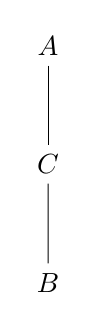
\begin{tikzpicture}[anchor=center]
		\node {$A$}
			child {node {$C$}
				child {node {$B$}}
			};
	\end{tikzpicture}
	};
	\node[inner, right=of pic a2] {
	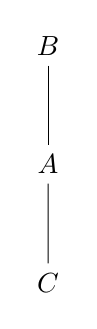
\begin{tikzpicture}[anchor=center]
		\node {$B$}
			child {node {$A$}
				child {node {$C$}}
			};
	\end{tikzpicture}
	};
\end{tikzpicture}
};

\node[outer, right=of pic a] (pic b) {
\begin{tikzpicture}
	\node[inner] (pic b1) {
	\begin{tikzpicture}[anchor=center]
		\node {$A$}
			child {node {$B$}
				child {node {$C$}}
			};
	\end{tikzpicture}
	};
	\node[inner, right=of pic b1] (pic b2) {
	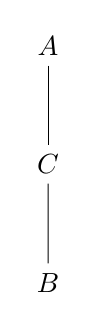
\begin{tikzpicture}[anchor=center]
		\node {$A$}
			child {node {$C$}
				child {node {$B$}}
			};
	\end{tikzpicture}
	};
	\node[inner, right=of pic b2.north east, anchor=north west] {
	\begin{tikzpicture}[anchor=center]
		\node {$A$}
			child {node {$B$}}
			child {node {$C$}};
	\end{tikzpicture}
	};
\end{tikzpicture}
};

\node[outer, right=of pic b] (pic c) {
\begin{tikzpicture}
	\node[inner] (pic c1) {
	\begin{tikzpicture}[anchor=center]
		\node {$A$}
			child {node {$B$}
				child {node {$C$}}
			};
	\end{tikzpicture}
	};
	\node[inner, right=of pic c1] (pic c2) {
	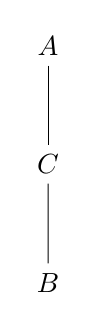
\begin{tikzpicture}[anchor=center]
		\node {$A$}
			child {node {$C$}
				child {node {$B$}}
			};
	\end{tikzpicture}
	};
	\node[inner, right=of pic c2.north east, anchor=north west] (pic c3) {
	\begin{tikzpicture}[anchor=center]
		\node {$A$}
			child {node {$B$}}
			child {node {$C$}};
	\end{tikzpicture}
	};
	\node[inner, right=of pic c3.north east, anchor=north west] {
	\begin{tikzpicture}[anchor=center]
		\node {$A$}
			child {node {$C$}}
			child {node {$B$}};
	\end{tikzpicture}
	};
\end{tikzpicture}
};

\node[draw=none, fill=none] (bottom center) at ($ (pic a.south west)!.5!(pic c.south east) $) {};

\node[outer, below=of bottom center, anchor=north] (pic d) {
\begin{tikzpicture}
	\node[inner] (pic d1) {
	\begin{tikzpicture}[anchor=center]
		\node {$A$}
			child[missing]
			child {node {$B$}
				child[missing]
				child {node {$C$}}
			};
	\end{tikzpicture}
	};
	\node[inner, right=of pic d1] (pic d2) {
	\begin{tikzpicture}[anchor=center]
		\node {$A$}
			child[missing]
			child {node {$B$}
				child {node {$C$}}
				child[missing]
			};
	\end{tikzpicture}
	};
	\node[inner, right=5mm of pic d2.north east, anchor=north west] (pic d3) {
	\begin{tikzpicture}[anchor=center]
		\node {$A$}
			child {node {$B$}}
			child {node {$C$}};
	\end{tikzpicture}
	};
	\node[inner, right=5mm of pic d3.north east, anchor=north west] (pic d4) {
	\begin{tikzpicture}[anchor=center]
		\node {$A$}
			child {node {$B$}
				child[missing]
				child {node {$C$}}
			}
			child[missing];
	\end{tikzpicture}
	};
	\node[inner, right=of pic d4] (pic d5) {
	\begin{tikzpicture}[anchor=center]
		\node {$A$}
			child {node {$B$}
				child {node {$C$}}
				child[missing]
			}
			child[missing];
	\end{tikzpicture}
	};
	\node[inner, below=of pic d1] (pic d6) {
	\begin{tikzpicture}[anchor=center]
		\node {$A$}
			child[missing]
			child {node {$C$}
				child[missing]
				child {node {$B$}}
			};
	\end{tikzpicture}
	};
	\node[inner, right=of pic d6] (pic d7) {
	\begin{tikzpicture}[anchor=center]
		\node {$A$}
			child[missing]
			child {node {$C$}
				child {node {$B$}}
				child[missing]
			};
	\end{tikzpicture}
	};
	\node[inner, right=5mm of pic d7.north east, anchor=north west] (pic d8) {
	\begin{tikzpicture}[anchor=center]
		\node {$A$}
			child {node {$C$}}
			child {node {$B$}};
	\end{tikzpicture}
	};
	\node[inner, right=5mm of pic d8.north east, anchor=north west] (pic d9) {
	\begin{tikzpicture}[anchor=center]
		\node {$A$}
			child {node {$C$}
				child[missing]
				child {node {$B$}}
			}
			child[missing];
	\end{tikzpicture}
	};
	\node[inner, right=of pic d9] {
	\begin{tikzpicture}[anchor=center]
		\node {$A$}
			child {node {$C$}
				child {node {$B$}}
				child[missing]
			}
			child[missing];
	\end{tikzpicture}
	};
\end{tikzpicture}
};

\foreach \x in {a,b,c,d} {
	\node[subpicture label, below=2mm of pic \x] {(\x)};
}

\end{tikzpicture}